\section{FFT Physical Optics - Multi Screen Propagation}
\textit{Consider a 1/2-screen model setup following [2]. Use some field conditioning described in [1]. Start with diffraction past one screen and look at behaviour around grazing incidence.}\\

\noindent \textit{A start of a program exercise\_MM9\_PO.m may be found at:}\\
\texttt{http://kom.aau.dk/\~pe/education/menu/9sem/}\\
\textit{Follow the ‘instructions'/ questions in the script and make it work and explain how/why.}\\


[1] \textit{Sections III \& IV of J. Walfisch \& H.L. Bertoni, "A Theoretical Model of UHF Propagation in Urban Environments", IEEE Trans. A\&P, vol. 36 no. 16, Dec 1988, pp. 1788-1796 (walfisch\_bertoni\_88.pdf)}\\

[2] \textit{Section II of J.-E. Berg \& H. Holmquist, "An FFT Multiple Half-Screen Diffraction Model", Proc . 44th IEEE VTC June 8th -10th 1994, Stockholm, Sweden, pp. 195-199 \\ (VTC94\_Berg\_Holmquist.pdf)}\\

To make the script work it was necessary to set an initial field of a propagating cylindrical wave.

\begin{flalign}
&&	E(r) =& \frac{e^{-jkr}}{\sqrt{r}}	&
\end{flalign}

Subsequently the field needed to be truncated to simulate in this way the effect of a fully absorbing screen. The truncated field must be zero in the absorbing screen. This field also needed to be neutralized using the neutralizer function from Walfisch and Bertoni.

The resulted field after the truncation and neutralization is shown in \figref{fig:mm11_one_screen}.

To calculate the field at the diffractive screen, according to the results of Berg and Holmquist, we can multiply the FFT of the incoming truncated and neutralized field by a propagator function (also defined in the $K_{y}$ domain) and then inverse Fourier transform to obtain the resulting field after the diffraction effect occurs. This propagator function in the $K_{y}$ domain appears because, in order to solve this diffraction problem one must solve the Helmholtz integral equation which for the actual geometry can be expressed as a convolution (Berg and Holmquist 1994). In \figref{fig:mm11_one_screen} one can appreciate the effect of the diffractive screen in the resulting field.


\begin{figure}[!h]
  \centering
  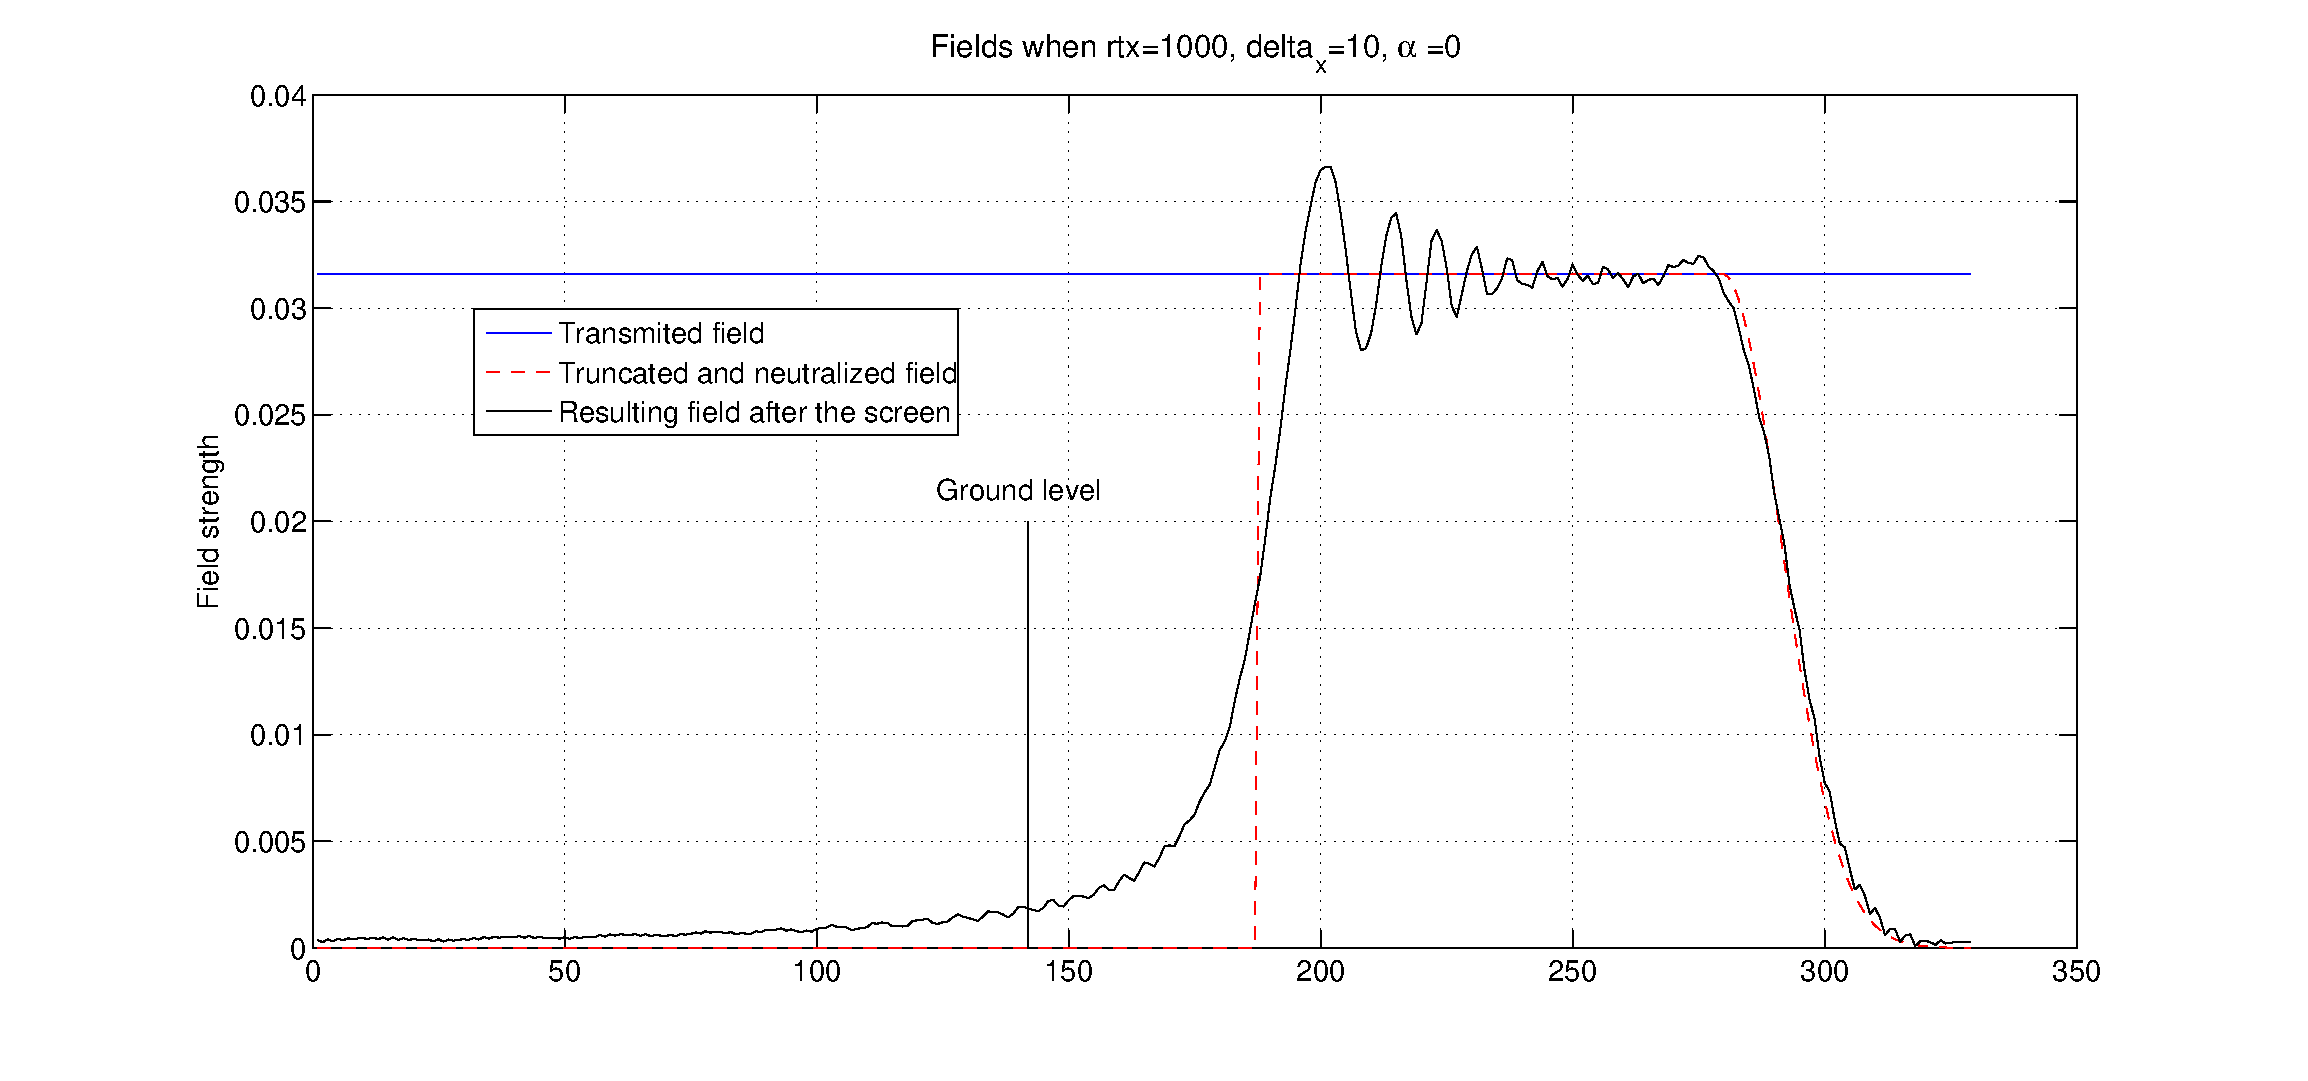
\includegraphics[width=16cm]{mm11_one_screen.eps}
  \caption{Plot showing the field received at the screen, the field truncated and neutralized with the neutralizer function and the resulting field after applying the propagator function}
  \label{fig:mm11_one_screen}
\end{figure}

This is an iterative method, which means that once we have found the resulting field after one diffractive screen, we can use it as an input for the next screen.